% Include architecture diagram and then subdivide each part of architecture as a
% section

\begin{figure*}[h!t]
  \centering
  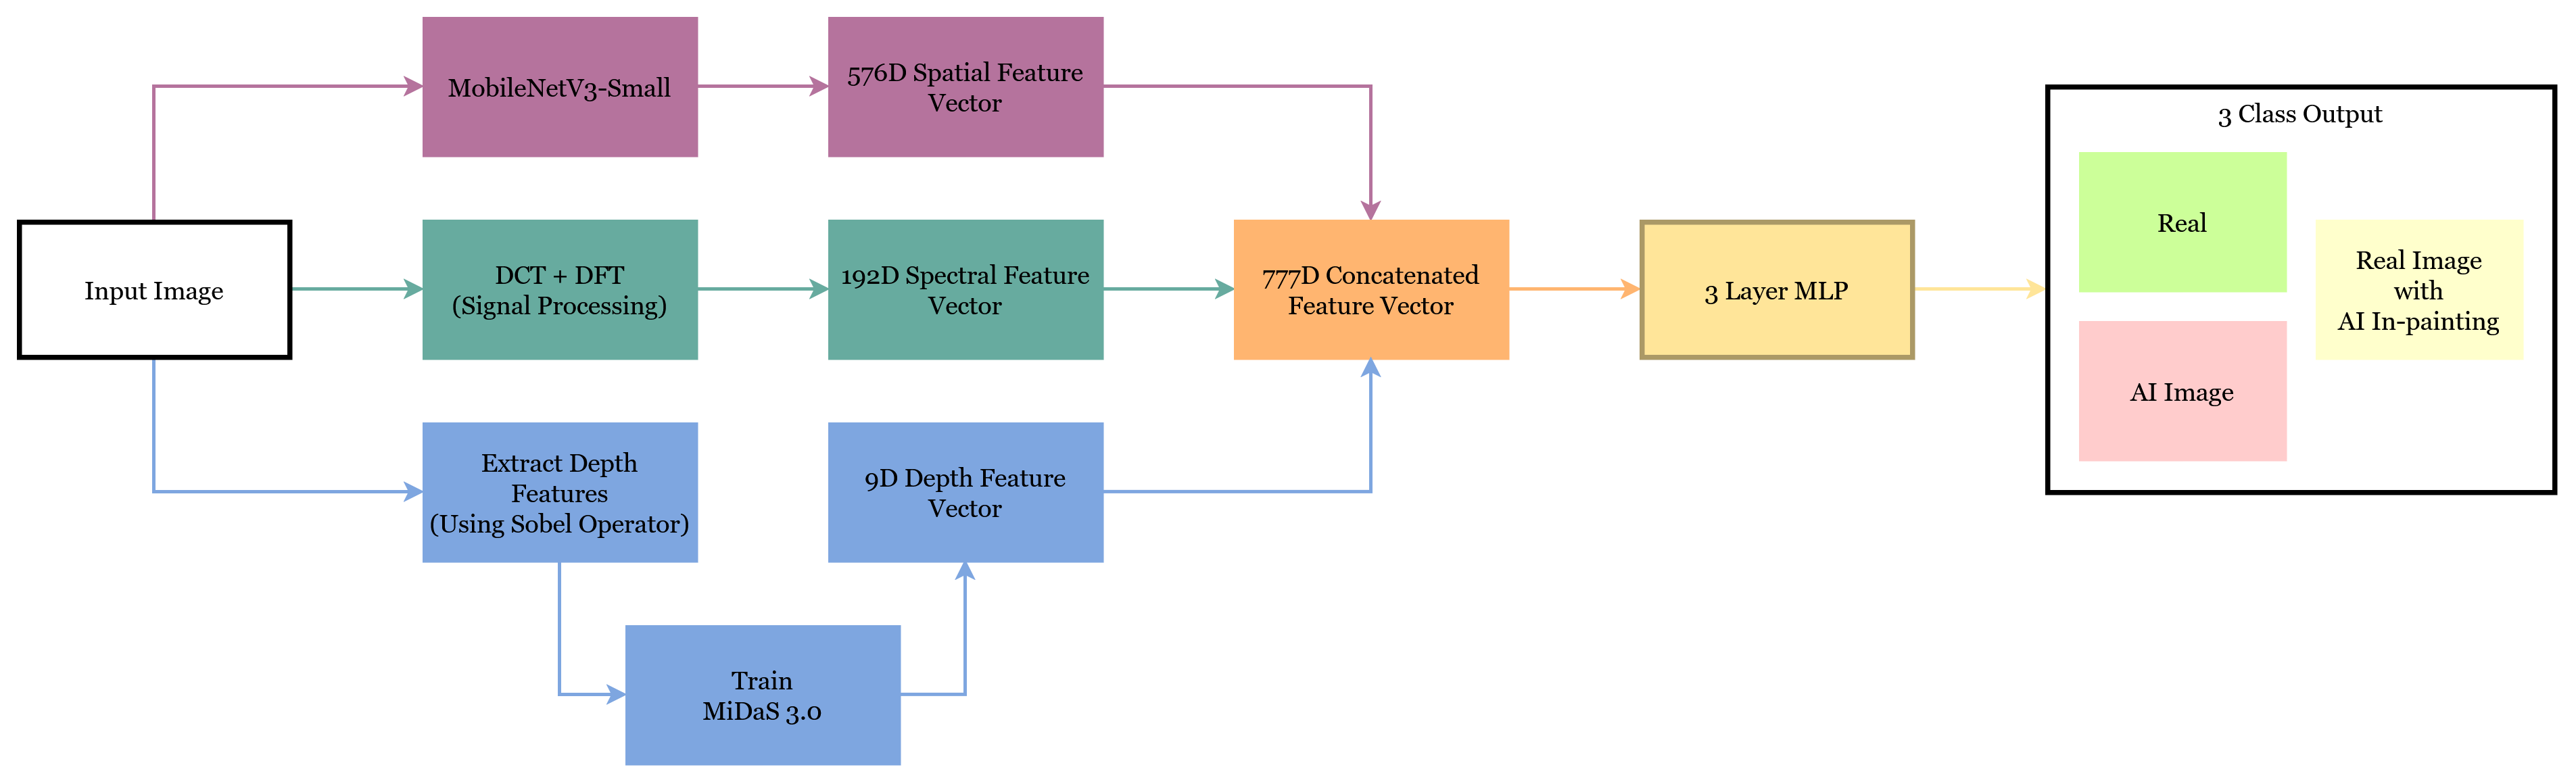
\includegraphics[width=\textwidth]{figs/pipeline.png}
  \caption{Pipeline of the Hybrid Framework explained in detail in the
    sections \ref{subsection:streama}, \ref{subsection:streamb} and
  \ref{subsection:streamc}.}
  \label {figure:pipeline}
\end{figure*}

Figure \ref{figure:pipeline} shows the brief architecture of the
proposed Multi-Domain Inconsistency Fusion (MDIF) framework. The
image will take three paths, combining spatial, spectral and
geometric inconsistencies to attain the lightweight hybrid detection pipeline.

The input image simultaneously goes through three independent streams:
\begin{enumerate}
  \item{Spatial Feature Stream}
  \item{Spectral Feature Stream}
  \item{Depth Consistency Stream}
\end{enumerate}
From which the extracted features are fused into a concatenated
representation, classified using a lightweight multilayer perceptron classifier.

\subsection{Stream A: Spatial Features} \label{subsection:streama}

The first path is to a Spatial RGB CNN, a MobileNetV3Small model
pretrained on ImageNet. The network extracts 576-dimensional spatial
feature vectors representing texture inconsistencies, abnormal
semantic structures, blending artifacts, overly-smoothed regions and
unrealistic object details.
MobileNetV3Small’s lightweight architecture and low computational
overhead makes it capable for strong feature extraction and suitable
for complex systems, often with resource constraints, adding to its
idealness for this framework.

\subsection{Stream B: Spectral Features} \label{subsection:streamb}

DCT (Discrete Cosine Transform) helps identify the smoothing
artifacts of the diffusion models along with periodic spectral
irregularities. The frequency of discontinuities across manipulated
regions and the loss of natural camera frequency distributions adds
onto DCT’s 192-dimensional spectral feature vector.
This frequency-domain analysis is key in detecting traces in low and
mid frequency components in images which AI generation may leave
behind, even when visual inspections are unable to identify them.

\subsection{Stream C: Depth Features} \label{subsection:streamc}

The final path is through the MiDaS model to generate a monocular
depth map. Gradient magnitude maps are computed from the RGB image
and the depth map using a Sobel-Feldman operator as seen in equation
\ref{eqn:sobel_feldman_grad_magnitude}. A consistency map
is created by computing the correlation scores from sliding a 16x16
window across the image. This is then used to create a 9-dimensional
discrepancy vector that captures the logically implausible
depth-shading relationships in images that diffusion models generate.

\begin{equation}
  \label{eqn:sobel_feldman_horizontal_changes}
  G_x =
  \begin{bmatrix}
    -1 & 0 & +1 \\
    -2 & 0 & +2 \\
    -1 & 0 & +1
  \end{bmatrix}
\end{equation}

\begin{equation}
  \label{eqn:sobel_feldman_vertical_changes}
  G_y =
  \begin{bmatrix}
    +1 & +2 & +1 \\
    0 & 0 & 0 \\
    -1 & -2 & -1
  \end{bmatrix}
\end{equation}

\begin{equation}
  \label{eqn:sobel_feldman_grad_magnitude}
  G = \sqrt{(G_x)^2 + (G_y)^2}
\end{equation}


AI-generated and inpainted images fail to maintain the realistic
depth and shading consistency in most cases, making this stream
effective in manipulation detection.

\subsection{Hybrid Classifier} \label{subsection:Hybrid}

These feature vectors are then concatenated to a 777-dimensional
feature vector which is  to a simple 3-Layer MLP (Multilayer
Perceptron) with ReLU activations and dropouts.
The final output will be a three-class probability distribution over
“Real”, “Fully AI Generated”, and “Real with AI Inpainting”.
